\documentclass{article}

\usepackage[left=2cm,top=1cm,right=2cm,bottom=2cm]{geometry}
\usepackage{hyperref}
\usepackage{graphicx}
\usepackage{tikz-cd}
\usepackage{amsmath}

\usepackage{listings}
 
\definecolor{codegreen}{rgb}{0,0.6,0}
\definecolor{codegray}{rgb}{0.5,0.5,0.5}
\definecolor{codepurple}{rgb}{0.58,0,0.82}
\definecolor{backcolour}{rgb}{0.95,0.95,0.95}
 
\lstdefinestyle{mystyle}{
    backgroundcolor=\color{backcolour},   
    commentstyle=\color{codegreen},
    keywordstyle=\color{magenta},
    numberstyle=\tiny\color{codegray},
    stringstyle=\color{codepurple},
    basicstyle=\small,
    breakatwhitespace=false,         
    breaklines=true,                 
    captionpos=b,                    
    keepspaces=true,                 
    numbers=left,                    
    numbersep=5pt,                  
    showspaces=false,                
    showstringspaces=false,
    showtabs=false,                  
    tabsize=2
}
 
\lstset{style=mystyle}

\renewcommand{\baselinestretch}{1.5}


\title{An Introduction To OpenSimRoot}
\author{Ernst Sch\"{a}fer}


\begin{document}

\maketitle

\tableofcontents

%\noindent This document aims to provide a comprehensive description of OpenSimRoot. We will address the following topics:
%\begin{itemize}
%\item The importance of modelling roots.
%\item The approach taken by the developers of OpenSimRoot.
%\item A technical discussion of the structure of OpenSimRoot.
%\item A guide to running simulations with OpenSimRoot.
%\item A guide to writing new modules.
%\item A comparison with other root simulation models.
%\end{itemize}

%%%%%%%%%%%%%%%%%%%%%%%%%%%%%%%%%%%%%%%
%\section{The Importance of Root Modelling.}
%
%\noindent Roots are vital to the functioning of all plants. Much of the research has been focused on the visible parts, with good reason. Root systems are notoriously difficult to study. Yet plants collect most of their much needed water and nutrient through their roots. Add to this the fact that soil degradation is increasingly common around the world and one can see why it is important to have a good understanding of root systems. \newline
%
%\noindent It is difficult to study roots during their lifetime, for obvious and less obvious reasons. Since roots are mostly found underground, they are far more difficult to keep track of than the shoot of a plant. A less obvious hurdle to understanding root systems is the existence of complex interactions between the root, micro-organisms and the soil. This is why root models are a useful tool to study the root system at intermittent stages of development. Once the necessary parameters have been determined from experiments and field studies, one can simulate many root systems under varying circumstances with relative ease. Simulations also allow us to study situations that are very rare in reality or focus on features that are difficult to determine. \newline
%
%\noindent An important area of current research is that of crops such as maize, wheat and bean. A lot of our food supply depends on these plants, yet there are still many aspects of their root systems we do not understand. Soil quality is poor in many places and using a lot of fertilizers is often not a sustainable option. We would like to understand the architectural traits that influence nutrient and water capture so we can select the phenotypes that will maximize yields under these poor conditions. \newline

\section{Foreword}

This document is by no means complete and very much a work in progress. It will, at some future time, include descriptions of all the core modules of OSR for which templates are available. These descriptions will list the dependencies, if any, the input parameters needed and the various options a module has. Based on user needs and feedback, new sections will be added and existing ones will be improved. Please contact the author at \href{ernst.schafer@nottingham.ac.uk}{ernst.schafer@nottingham.ac.uk} with any requests or queries.

\section{Introduction}

\noindent It is obvious that a plant can increase its uptake of nutrients and water by growing a more expansive root system. However, the costs associated with growing and maintaining a root system mean that plants can not simply grow as many roots as they would like. The size of the root system is constrained by, among other things, the amount of available resources. This means that plants have to weigh the costs of their root systems against the benefits they provide. OpenSimRoot aims to model the three-dimensional structure of the root system, the water and nutrient uptake by the roots, the water and nutrient flow in the soil and, perhaps most importantly, the carbon costs associated with growing and maintaning a root system and taking up the nutrients needed by the plant \cite{Postma2017}. By keeping track of the costs associated with growing and maintaining a root system, OpenSimRoot is able to compare the resource efficiency of different architectures in different environments. Here resource efficiency is defined as 

$$E = \frac{\sum_{n} \frac{U_n}{R_n}}{C_r} $$

\noindent where $E$ is the resource efficiency, $U_n$ the total uptake of nutrient $n$ by the root system, $R_n$ the amount of nutrient $n$ needed for metabolism and growth and $C_r$ the fraction of total carbon produced that is spent on the root system. \newline

\noindent For example, using OpenSimRoot, Postma et al. \cite{Postma2014} found that the optimal lateral root branching density depends on the availability of nitrogen and phosphorus. Inter-root competition for mobile resources such as nitrogen lead to diminishing returns on investment in lateral roots. Since the amount of carbon a plant can allocate is fixed by the shoot, higher lateral root branching density implies that the laterals are shorter, thus decreasing the efficiency. In contrast, for highly immobile nutrients such as phosphorus, there is far less competition between roots so a higher lateral root density is the more efficient architecture. Field trials show a median lateral branching density between these two extremes, suggesting that plants are finding an optimum between them. This example highlights the power of simulation in not only explaning certain features seen in field trials but also generating new questions for experimentalists. \newline

%%%%%%%%%%%%%%%%%%%%%%%%%%%%%%%%%%%%%%%
\section{The Structure of OpenSimRoot}

\noindent OpenSimRoot is written in C++. It consists of different modules and allows the user to choose which modules to include in the simulation (though the dependency between modules imposes some restriction on the possible choices). This allows the user to study only the aspects of interest without the computational effort of running every module. The basis for OpenSimRoot is what is called the extensible tree structure. This captures not only the topology of the root system, but also provides a way to link properties to roots. Before we explain this in more detail, we will first explain in broad strokes how the engine of OpenSimRoot works. OpenSimRoot does not currently have a graphical user interface and must be run through the command line (or terminal if you're a linux or mac user).

\subsection{The Engine}\label{Engine}

\noindent Let us first fix some definitions:

\begin{itemize}
\item \textbf{Minimodel.} A minimodel is, simply put, a state variable, which often depends on space and/or time. Minimodels derive from \textbf{SimulaBase}. The value of a minimodel can be requested through the application programming interface (API), which is described in more detail in section \ref{API}.
\item \textbf{Plugin.} A plugin is a class that computes the values of a minimodel. Plugins derive from \textbf{DerivativeBase}. Plugins obtain information through the API and use this to compute new values.
\item \textbf{Module.} We will refer a set of classes that, together, simulate a certain aspect of reality, as a module. This will involve at least one plugin and one minimodel.
\end{itemize}

\noindent As mentioned above, the information of the model is contained in the minimodels while the plugins do the calculations necessary for updating them. Each plugin is known by an unique name that the user refers to in the XML input files (see section \ref{Input}), to specify what plugin (function) OpenSimRoot should use to calculate the value of a minimodel. This allows the user to run a simulation using different plugins for the same state variable and compare results. The values of minimodels are only calculated when requested through the API. The simulation is advanced forward in time by virtue of the export modules which start requesting the data needed for output when they are initiated. \newline

\noindent All the minimodels derive from a class of the form \textbf{SimulaX} and these derive from \textbf{SimulaBase} (except \textbf{SimulaBase} itself of course). The \textbf{SimulaBase} class implements all general methods used to send and request information, making up the API. The derived classes each implement some methods and/or members needed when using that object type. The inheritance of the \textbf{SimulaX} classes is summarized in figure 1.
\begin{center}
\begin{figure}[h!]
\begin{tikzcd}[column sep=tiny]
& & \textbf{SimulaBase} \arrow[dll] \arrow[dl] \arrow[d] \arrow[dr] \arrow[drr] \arrow[r, leftrightarrow] & \textbf{Database} & \\
\textbf{SimulaConstant} & \textbf{SimulaDynamic} \arrow[dl] \arrow[d] \arrow[dr] & \textbf{SimulaGrid} & \textbf{SimulaLink} & \textbf{SimulaStochastic} \\
\textbf{SimulaDerivative} & \textbf{SimulaTable} & \textbf{SimulaTimeDriven} \arrow[dl] \arrow[d] \arrow[dr] & & \\
& \textbf{SimulaExternal} & \textbf{SimulaPoint} & \textbf{SimulaVariable} & 
\end{tikzcd}
\caption{Inheritance of the \textbf{SimulaX} classes. The arrow between \textbf{SimulaBase} and \textbf{Database} signifies that \textbf{Database} is privately owned by \textbf{SimulaBase}. The other arrows indicate inheritance of classes.}
\end{figure}
\end{center}

%%\noindent We can briefly summarize the use of each class as follows. \newline
 
%% \begin{itemize}
%%\item \textbf{SimulaBase} contains the methods needed for the API and basic members needed by every state variable.
%%\item \textbf{SimulaConstant} is used for constants.
%%\item \textbf{SimulaDynamic} is used for variables that change in time.
%%\item \textbf{SimulaGrid} is used to encode a grid of values with an interpolation algorithm.
%%\item \textbf{SimulaLink} provides a connection to a different minimodel.
%%\item \textbf{SimulaStochastic} is used for a random variable drawing from a given distribution.
%%\item \textbf{SimulaDerivative} contains a plugin, which is derived from \textbf{DerivativeBase} (the plugin, not \textbf{SimulaDerivative}).
%%\item \textbf{SimulaTable} is used to provide input values that change over time. The data is interpolated if needed.
%%\item \textbf{SimulaTimeDriven} is used for certain variables changing over time.
%%\item \textbf{SimulaExternal} is used to obtain values from other simulation models.
%%\item \textbf{SimulaPoint} is used to describe a point moving through space.
%%\item \textbf{SimulaVariable} is used to simulate a variable changing over time using numerical integration.
%%\item \textbf{Database.} This class keeps track of all the minimodels in the simulation.
%%\end{itemize}

\noindent For a brief explanation of each of these classes, see section \ref{Input}. All the minimodels are linked together in what is called the extensible tree structure (ETS). This is a structure that both reflects the physical structure of the root system as well as the connections between different properties. In the most basic terms, it is a set of objects, arranged in a hierarchy with pointers to certain other objects. Each object has one \textit{parent} and might have one or more \textit{children}. Objects can be added and removed dynamically as needed. The XML input files also follow this structure.\newline
 
%\noindent {\color{red}The name extensible tree structure gives a hint of what this structure looks like. Think of it as a set of objects organized in something like a family tree. Each object (apart from the \textit{origin}-object) has one parent and might have some children. Examples of these objects are plants that are simulated, the shoot, a single root, a root segment or some module. Each object contains pointers to its parent, children and siblings. Using this one can calculate functions that depend on the entire root system with relative ease. For example, should one desire to know the total root length, one simply calls the totalRootLength module. This module is attached to the plant object and will get the rootLength of each individual root, which in turn is calculated by calling the rootSegmentLength objects attached to all the datapoints that make up the root. \newline
%
%\noindent This structure is reflected in the input files as well which should be XML files. The xml format is similar to html in that it is a markup language. The xml format allows the user to define tags which contain certain data. The tags in OpenSimRoot input files must specify the plant, the soil, which modules are in use and the values of parameters needed for the simulation. The tags generally fall in the categories: parameters, containers and functions/modules. A parameter tag is easy to understand, it contains a parameter such as the growth rate of a root. Containers are tags that define places in the initial extensible tree structure where OpenSimRoot will place certain objects it creates. For example, each root has a child called \textit{datapoints} that contains all the datapoints, which are more or less the segments of the root. There are also tags that couple a name to a function/module. If they encode information about the whole plant, such as the total root length, they will be included in the output table by OpenSimRoot. If they encode information about smaller parts of the plant, such as the diameter of a root segment, they will be included in the 3D data. We will provide a more comprehensive description in the next chapter. \newline
%
%\noindent An important aspect of OpenSimRoot is that it can model many different root classes, each with their own properties. Examples are the primary root, brace roots, seminal roots, lateral roots and, if required, sublateral roots, subsublateral roots etc. Each root type can have different branching parameters, growth rates, gravitropism, etc. This does mean that all these parameters need to be specified for all root types that are included in the simulation. By specifying different branching rules and growth rates, a wide variety of root systems can be simulated. \newline
%
%\noindent As stated before, the only way to get a value from a class, is through the \textbf{get} method which will call the \textbf{calculate} method of the class. Some of the most important classes are}

%%%%%%%%%%%%%
\subsection{The Modules}

In this section we will briefly explain the workings of some important modules in OpenSimRoot. \newline

\noindent In OpenSimRoot each root is simulated as a number of vertices connected by edges. One of these vertices has time-dependent coordinates, it is called the growthpoint. The speed of the growthpoint is defined by the base growth rate specified in the XML input file and some correction factors that might relate to various stresses and conditions. The direction in which the growth point moves is determined according to some rules relating to gravitropism, the emergence angle of roots and a stochastic contribution. The other vertices have static locations and are placed in the path of the growthpoint as it moves. The root length is the distance the growthpoint travelled, not the sum of the distances between the vertices. \newline

\noindent New roots are created according to branching rules which specify the distance or time between subsequent branchings. Branches emerge from what are called xylem poles, the number of xylem poles determines the radial angles at which new branches can emerge. The XML input file specifies both the axial branching angle as well as the types of roots that can branch from a certain root class. Each root class has their own parameters, such as growth rates, branching rates, etc. \newline

\noindent OpenSimRoot contains a simple, abstract shoot model in which the shoot is represented by a number of variables. A simple photosynthesis model determines the rate of carbon production based on the leaf area and the carbon fixation rate. The carbon requirements are based on the growth and respiration rates of the roots, costs associated to root exudates and nitrate uptake and the requirements of the shoot. If the amount of produced carbon is greater than the amount required, leftover carbon is stored in a labile pool for later use. If the amount of produced carbon is smaller than the amount required, root growth rates decline. \newline

\noindent The hydrology module in OpenSimRoot consists of three models that are linked together. One is a simplified implementation of the SWMS model in C++ which simulates water transport through the soil by numerically solving the Richards' equation \cite{Simunek1995}. The Richards' equation is:

$$ \frac{\partial \theta}{\partial t} = \nabla \left[ K(\theta)\nabla ( h(\theta) + z) \right] - S $$

\noindent Here $\theta$ is the volumetric water content, $t$ is time, $K(\theta)$ is the hydraulic conductivity tensor, $h(\theta)$ is the matrix head, $z$ is the elevation above some reference point and $S$ is a sink term that represents the water uptake by roots. Evapotranspiration, which is a term that includes the evaporation of water from the soil and transpiration by the plants, is simulated by the Penman-Monteith equation \cite{Allen1998, Monteith1965, Monteith1981, Penman1948}. The transport of water through the xylem is simulated by the hydraulic network model \cite{Alm1992, Doussan1998}. \newline

\noindent The transport of nutrients in the soil is simulated with convection-diffusion equations for which there are currently two implementations in OpenSimRoot. One is the one-dimensional Barber-Cushman model that is used to simulate depletion zones around root segments \cite{Itoh1983}. The second is an implementation of the solute model in SWMS3D that couples to the water transport model \cite{Simunek1995}. The uptake of nutrients by the root system is modelled with Michaelis-Menten kinetics. The nutrient uptake rate of a root segment, $I_n$, is equal to

$$ I_n = \begin{cases} \frac{I_{max}(C-C_{min})}{K_m + C - C_{min}} & \hspace{10pt} \text{if} \hspace{10pt} C \geq C_{min} \\ 0 & \hspace{10pt} \text{if} \hspace{10pt} C< C_{min} \end{cases} $$

\noindent Here $I_{max}$ is the maximal uptake rate of the root segment, $C$ is the nutrient concentration at the root surface, $C_{min}$ is the minimal nutrient concentration at which the root segment can take up nutrients and $K_m$ is the concentration at which $I = \frac{I_{max}}{2}$. If the amount of nutrients taken up is smaller than what is optimal, the plant undergoes a stress response. This can impact growth rates, photosynthesis rates and respiration rates. Nutrients and water are, in the current version, distributed instantly and uniformly around the plant, so every organ experiences the same stress. Mineralisation is modelled by the Yang-Janssen model \cite{Yang2000}. \newline

%%%%%%%%%%%%%%%%%%%%%%%%%%%%%%%%%%%%%%%
\section{Downloading and Running OpenSimRoot}

We will describe how to download, install and run OpenSimRoot. This section is aimed at developers, there will be a standalone executable at some point in the future. The terminal commands in this section were run on a Linux machine but should be the same on Mac and Windows systems, unless explicitly stated otherwise. Example input files can be found in the \href{https://gitlab.com/rootmodels/OpenSimRoot}{OSR online repository}. In the next section we will describe the structure input files should have. First of all, if you do not know what Git is, it's advisable to check out a short introduction \href{https://speakerdeck.com/alicebartlett/git-for-humans}{here}. \newline

\noindent We will make a local copy of the OpenSimRoot repository (this is called \textit{cloning}) and \textit{build} it (we create an executable that we can run). First create an account on gitlab.com and make sure you have access to the OpenSimRoot repository. Then check if Git is installed. Do this by entering: \verb|git --version|. Your output should be of the form: \verb|git version 1.8.3.1|. If Git is not installed, see: \url{https://git-scm.com/book/en/v2/Getting-Started-Installing-Git} \newline

\noindent Now we will add the user name and email. We do this by entering the commands:
\begin{verbatim}
git config --global user.name USERNAME
git config --global user.email EMAIL ADDRESS
\end{verbatim}

\noindent You can check if they were entered correctly by entering: \verb|git config --global --list|. Now copy the HTTPS url of the online repository from the \href{https://gitlab.com/rootmodels/OpenSimRoot}{OSR Gitlab page}. It can be found on the main page of the repository, there is a text box near the top of the page with a drop-down menu beside it which is set to SSH by default. The SSH address is \verb|git@gitlab.com:rootmodels/OpenSimRoot.git| at the time of writing. Change SSH to HTTPS and copy the link, which at the time of writing is \verb|https://username@gitlab.com/rootmodels/OpenSimRoot.git|. \verb|cd| to the directory that you want your local repository to end up in, \verb|home/git| for example, and enter \verb|git clone| followed by the HTTPS url. It will probably look like:
\begin{verbatim}
git clone https://username@gitlab.com/rootmodels/OpenSimRoot.git
remote: Counting objects: 1345, done.
remote: Compressing objects: 100% (418/418), done.
remote: Total 1345 (delta 863), reused 1328 (delta 855)
Receiving objects: 100% (1345/1345), 2.00 MiB | 2.54 MiB/s, done.
Resolving deltas: 100% (863/863), done.
Checking out files: 100% (310/310), done.
\end{verbatim}
%Now we need an SSH key. Check if there is an existing key by entering: \verb|cat ~/.ssh/id_rsa.pub| If there is no key, make one by entering: \verb|ssh-keygen -t rsa -C "EMAIL ADDRESS"| (the quotes are important!). Next you will be asked to enter a filename in which the key will be saved. Leave it blank to use the default name (recommended). After this you will be asked to enter a passphrase. It is recommended that you do this but you can leave it empty to make a key without passphrase. Now you should see a message stating the key has been saved, a key fingerprint and a randomart image. Type in the following command to see the key: \verb|cat ~/.ssh/id_rsa.pub| \newline
%
%\noindent If you saved the key in a different directory, change \verb|~| accordingly. If you changed the filename, change \verb|id_rsa.pub| accordingly. The key should start with: \verb|ssh-rsa| and end with your email address. Copy all of it and enter it in the appropriate text box on: \url{https://gitlab.com/profile/keys}. Choose a name for the key and save it. \newline
%
%% \noindent Create an empty git repository with \verb|git init|. \newline
%
%\noindent Now go to: \url{https://gitlab.com/rootmodels/OpenSimRoot} and copy the SSH address to your clipboard. In your terminal, go to the directory you want to create your local copy of OpenSimRoot in and enter:\\
%\verb|git clone THE SSH ADDRESS YOU COPIED| \\ 
%At the time of writing the command is: \verb|git clone git@gitlab.com:rootmodels/OpenSimRoot.git| \\
%You might get a message stating that:\\ 
%\verb|The authenticity of host 'gitlab.com (104.210.2.228)' can't be established.| \\
%Enter \verb|yes| to continue. Now the files will be copied and you will see:

\noindent Now there should be a new directory called OpenSimRoot with all the files in it. Next we will set up our remote repository. We do this by changing directory to the OpenSimRoot directory we just created and entering the command:
\verb|git remote add origin git@gitlab.com:rootmodels/OpenSimRoot.git| \newline

\noindent This tells git to add a remote, with the name \textit{origin} and with as source the SSH address of the OpenSimRoot repository. You can check the remotes you added with their names with: \verb|git remote -v|. Now whenever we want to get the latest version we make sure we are in the OpenSimRoot directory and enter: \verb|git pull origin|. This tells git to \verb|fetch| and then \verb|merge|. The \verb|fetch| command copies the latest changes from the repository and \verb|merge| then merges these changes with the local copy of the repository. In order to avoid conflicts it is a good idea to \verb|pull| before any local changes are made. \newline

\noindent For more on remotes, see: \url{https://help.github.com/categories/managing-remotes/}. For the difference between fetch and pull see: \\
 \url{http://stackoverflow.com/questions/292357/what-are-the-differences-between-git-pull-and-git-fetch}

\begin{verbatim}
[pmxeds@kazbek OpenSimRoot]$ git remote add origin git@gitlab.com:rootmodels/OpenSimRoot.git
[pmxeds@kazbek OpenSimRoot]$ git fetch origin 
remote: Counting objects: 3, done.
remote: Compressing objects: 100% (3/3), done.
remote: Total 3 (delta 2), reused 0 (delta 0)
Unpacking objects: 100% (3/3), done.
From gitlab.com:rootmodels/OpenSimRoot
 * [new branch]      master     -> origin/master
 * [new branch]      osx-r\bibliography{../Articles/Database}{}
\bibliographystyle{plain}edirect -> origin/osx-redirect
\end{verbatim}

\noindent When you tell git to pull you might get the following error message:

\begin{verbatim}
[pmxeds@kazbek OpenSimRoot]$ git pull origin
You asked to pull from the remote 'origin', but did not specify
a branch. Because this is not the default configured remote
for your current branch, you must specify a branch on the command line.
\end{verbatim}

\noindent This means you have not specified a default branch for your current branch (the default branch is master). You can do this by entering: \verb|git branch --set-upstream-to origin/master|. This will set the master branch of the remote repository (assuming you called it origin) as the default branch for your current branch (which should be your master branch). Now you can use \verb|git push| and \verb|git pull| without specifying the branch. To see what has been changed, use: \verb|git diff master@{1} master| (substituting a higher integer for 1 allows you to look further back in time). Now you should get:

\begin{verbatim}
[pmxeds@kazbek OpenSimRoot]$ git pull origin
Already up-to-date.
\end{verbatim}

\noindent We will build OpenSimRoot with gcc, which is a compiler. To see if gcc is installed, enter the commands stated below and see if the output is similar.
\begin{verbatim}
[pmxeds@kazbek ~]$ whereis gcc
gcc: /usr/bin/gcc /usr/lib/gcc /usr/libexec/gcc /usr/share/man/man1/gcc.1.gz
[pmxeds@kazbek ~]$ which gcc
/usr/bin/gcc
[pmxeds@kazbek ~]$ gcc --version
gcc (GCC) 4.8.5 20150623 (Red Hat 4.8.5-4)
Copyright (C) 2015 Free Software Foundation, Inc.
This is free software; see the source for copying conditions.  There is NO
warranty; not even for MERCHANTABILITY or FITNESS FOR A PARTICULAR PURPOSE.
\end{verbatim}

\noindent For more on gcc, see: \url{http://www.cyberciti.biz/faq/howto-compile-and-run-c-cplusplus-code-in-linux/}. Now change directory to OpenSimRoot/OpenSimRoot/StaticBuild by using \verb|cd|

\begin{verbatim}
[pmxeds@kazbek ~]$ cd OpenSimRoot
[pmxeds@kazbek OpenSimRoot]$ ls
build.sh         executeBeforeCommitToTest.sh  public             runTestsModules.sh
cleanup.sh       LICENSE                       README.md          runTests.sh
OpenSimRoot      runTestsEngine.sh             warnings.txt
\end{verbatim}

\noindent Now enter the command \verb|bash build.sh| (Linux and Mac) or \verb|cd| to \verb|OpenSimRoot/StaticBuild| and use \verb|make all| (Windows). Gcc will now build opensimroot. After a while you will see: \\ \verb|Finished building target: OpenSimRoot|. \\

\noindent Execute: \verb|OpenSimRoot/StaticBuild/OpenSimRoot -h| to check if everything is correct. You will get the output:

\begin{verbatim}
[pmxeds@kazbek StaticBuild]$ ./OpenSimRoot -h
Usage: OpenSimRoot [OPTIONS] [FILE]
OpenSimRoot simulates a model defined in FILE

  -f, --file                 specify simulation file, default last argument
  -h, --help or /?           print this help message
  -v                         be verbose with warnings
  -q                         be quite with warnings
  -l, --list                 print list of registered functions
  -V, --verify               Experimental function for verifying input files

Examples:
  OpenSimRoot -h             Prints this message
  OpenSimRoot runModel.xml   Runs the OpenSimRoot model 

Support at j.postma@fz-juelich.de
Licensed to you under the GPLv3 license.

There are no warnings.
Simulation took (hours:minutes:seconds): 0:0:0
\end{verbatim}

\noindent Now test the engine and modules with the command \verb|bash runTests.sh|. You should get the following output:

\begin{verbatim}
[pmxeds@kazbek OpenSimRoot]$ bash runTests.sh 
Testing engine
using ../../StaticBuild/OpenSimRoot as exe
Test SimulaConstant.xml passed
Test SimulaTable.xml passed
Test SimulaGrid.xml passed
Test SimulaVariable.xml passed
Test SimulaPoint.xml passed
Test SimulaStochastic.xml passed
Done running tests, comparing results
Done
finished testing engine with error status 0
Testing modules
Testing OneSimpleStraightRoot.xml
using ../../StaticBuild/OpenSimRoot as exe
Test OneSimpleStraightRoot.xml passed
Test PartiallyPredefinedBranchedRoot.xml passed
Test Barber-Cushman.xml passed
Test SimpleCropModel.xml passed
Done running testing modules, comparing results
Done
finished testing engine with error status 0
exiting with error status 0
\end{verbatim}

\noindent For a more comprehensive guide on some of the steps involved see: \\
\url{https://gitlab.com/help/gitlab-basics/README.md} \newline

\noindent We will describe how to run a simulation with OpenSimRoot. First it is important to know how OpenSimRoot operates. OpenSimRoot takes as input an XML file. This file contains the parameters for the simulation you want to run. This includes parameters like: The duration of the simulation, the environmental parameters, the initial root structure, the properties of the different types of roots etc. OpenSimRoot uses this data to run the simulation and then gives the output that the user has requested. This output can consist of aggregated variables, like the total root length, the amount of water/nitrogen depleted from the soil but OpenSimRoot can also put out files that, for example, contain the entire root structure at each day. This can be viewed by ParaView. As a sidenote, it is possible to specify an entire root structure (with the appropriate time parameters) which OpenSimRoot will then grow. This can be used to compare the simulated results to a real result. \newline

\noindent First we choose an output directory. It is strongly advised you make separate directories for OpenSimRoot, the XML files you will use as input and your output. While this requires you to enter slightly longer file paths in the terminal, your files will be much more organized. In the directory \verb|OpenSimRoot/OpenSimRoot/InputFiles| there are some example XML files which we will try to run. \newline

\noindent Use cd to move to the output directory, which we assume is \verb|home/git/OpenSimRootOutputs|. Since our \textit{OpenSimRoot} directory is \verb|home/git/OpenSimRoot|, this would be:
\begin{verbatim}
cd ../OpenSimRootOutputs
\end{verbatim}

\noindent We make a folder where we will output our test results with \verb|mkdir Test| and then \verb|cd Test|. Now we will tell OpenSimRoot to open the file \textit{runStraightRoot.xml} by executing (don't copy the line break!): 
\begin{verbatim}
../../OpenSimRoot/OpenSimRoot/StaticBuild/OpenSimRoot -f
../../OpenSimRoot/OpenSimRoot/InputFiles/runStraightRoot.xml
\end{verbatim}

\noindent The first part is the path to the OpenSimRoot executable. \verb|-f| tells OpenSimRoot that we want to open a file. The last part is the path to the file we want to take as input. After the simulation is complete, the \textit{Test} directory contains (depending on what was specified) files  called: \textit{tabled\_output.tab}, \textit{warnings.txt}, some .vtu files and some .pvd files. The \textit{tabled\_output.tab} contains the values of variables like the nitrogen depletion, the dry weight of the plant and the total root length on each day (again depending on what output was specified). \textit{warnings.txt} has an obvious meaning. The .vtu and .pvd files contain spatial information on the soil and root system and can be visualized with ParaView. \newline

\noindent To do this, open ParaView (\verb|paraview|) and open \textit{VisualizationRoots.pvd} (\textit{file}$\rightarrow$\textit{open}), then click \textit{Apply} in the \textit{Properties} window on the left. You will probably not see anything because at time t=0 there is no root structure yet! Click the \textit{Play} button in the top bar and you will see the root structure as it is growing. By default, the root structure is uniformly coloured so this only shows us the topology of the root system. To see more relevant information, in the properties window on the left, under the header \textit{Coloring}, select something else instead of \textit{Solid Color} to see the property you selected coloured (in the example below I chose rootClassID). By default the \textit{Color Space} option (in the \textit{Color Map Editor} on the right) is set to \textit{Diverging}, some other colour map will probably suit you better. You can choose a different colour mapping and alter the sensitivity by adjusting the circles and curve in the \textit{Mapping Data} section on the right. Double click on a circle in the bar at the bottom to choose a different colour. \newline

\noindent It is also possible to see the depletion of nutrients in the soil, assuming OpenSimRoot was told to output this, by also opening the \textit{fem.pvd} file. \newline

\noindent See the following picture for a sample visualization where the different colours indicate different types of roots (primary, seminal, lateral).

\begin{figure}[h]
\begin{center}
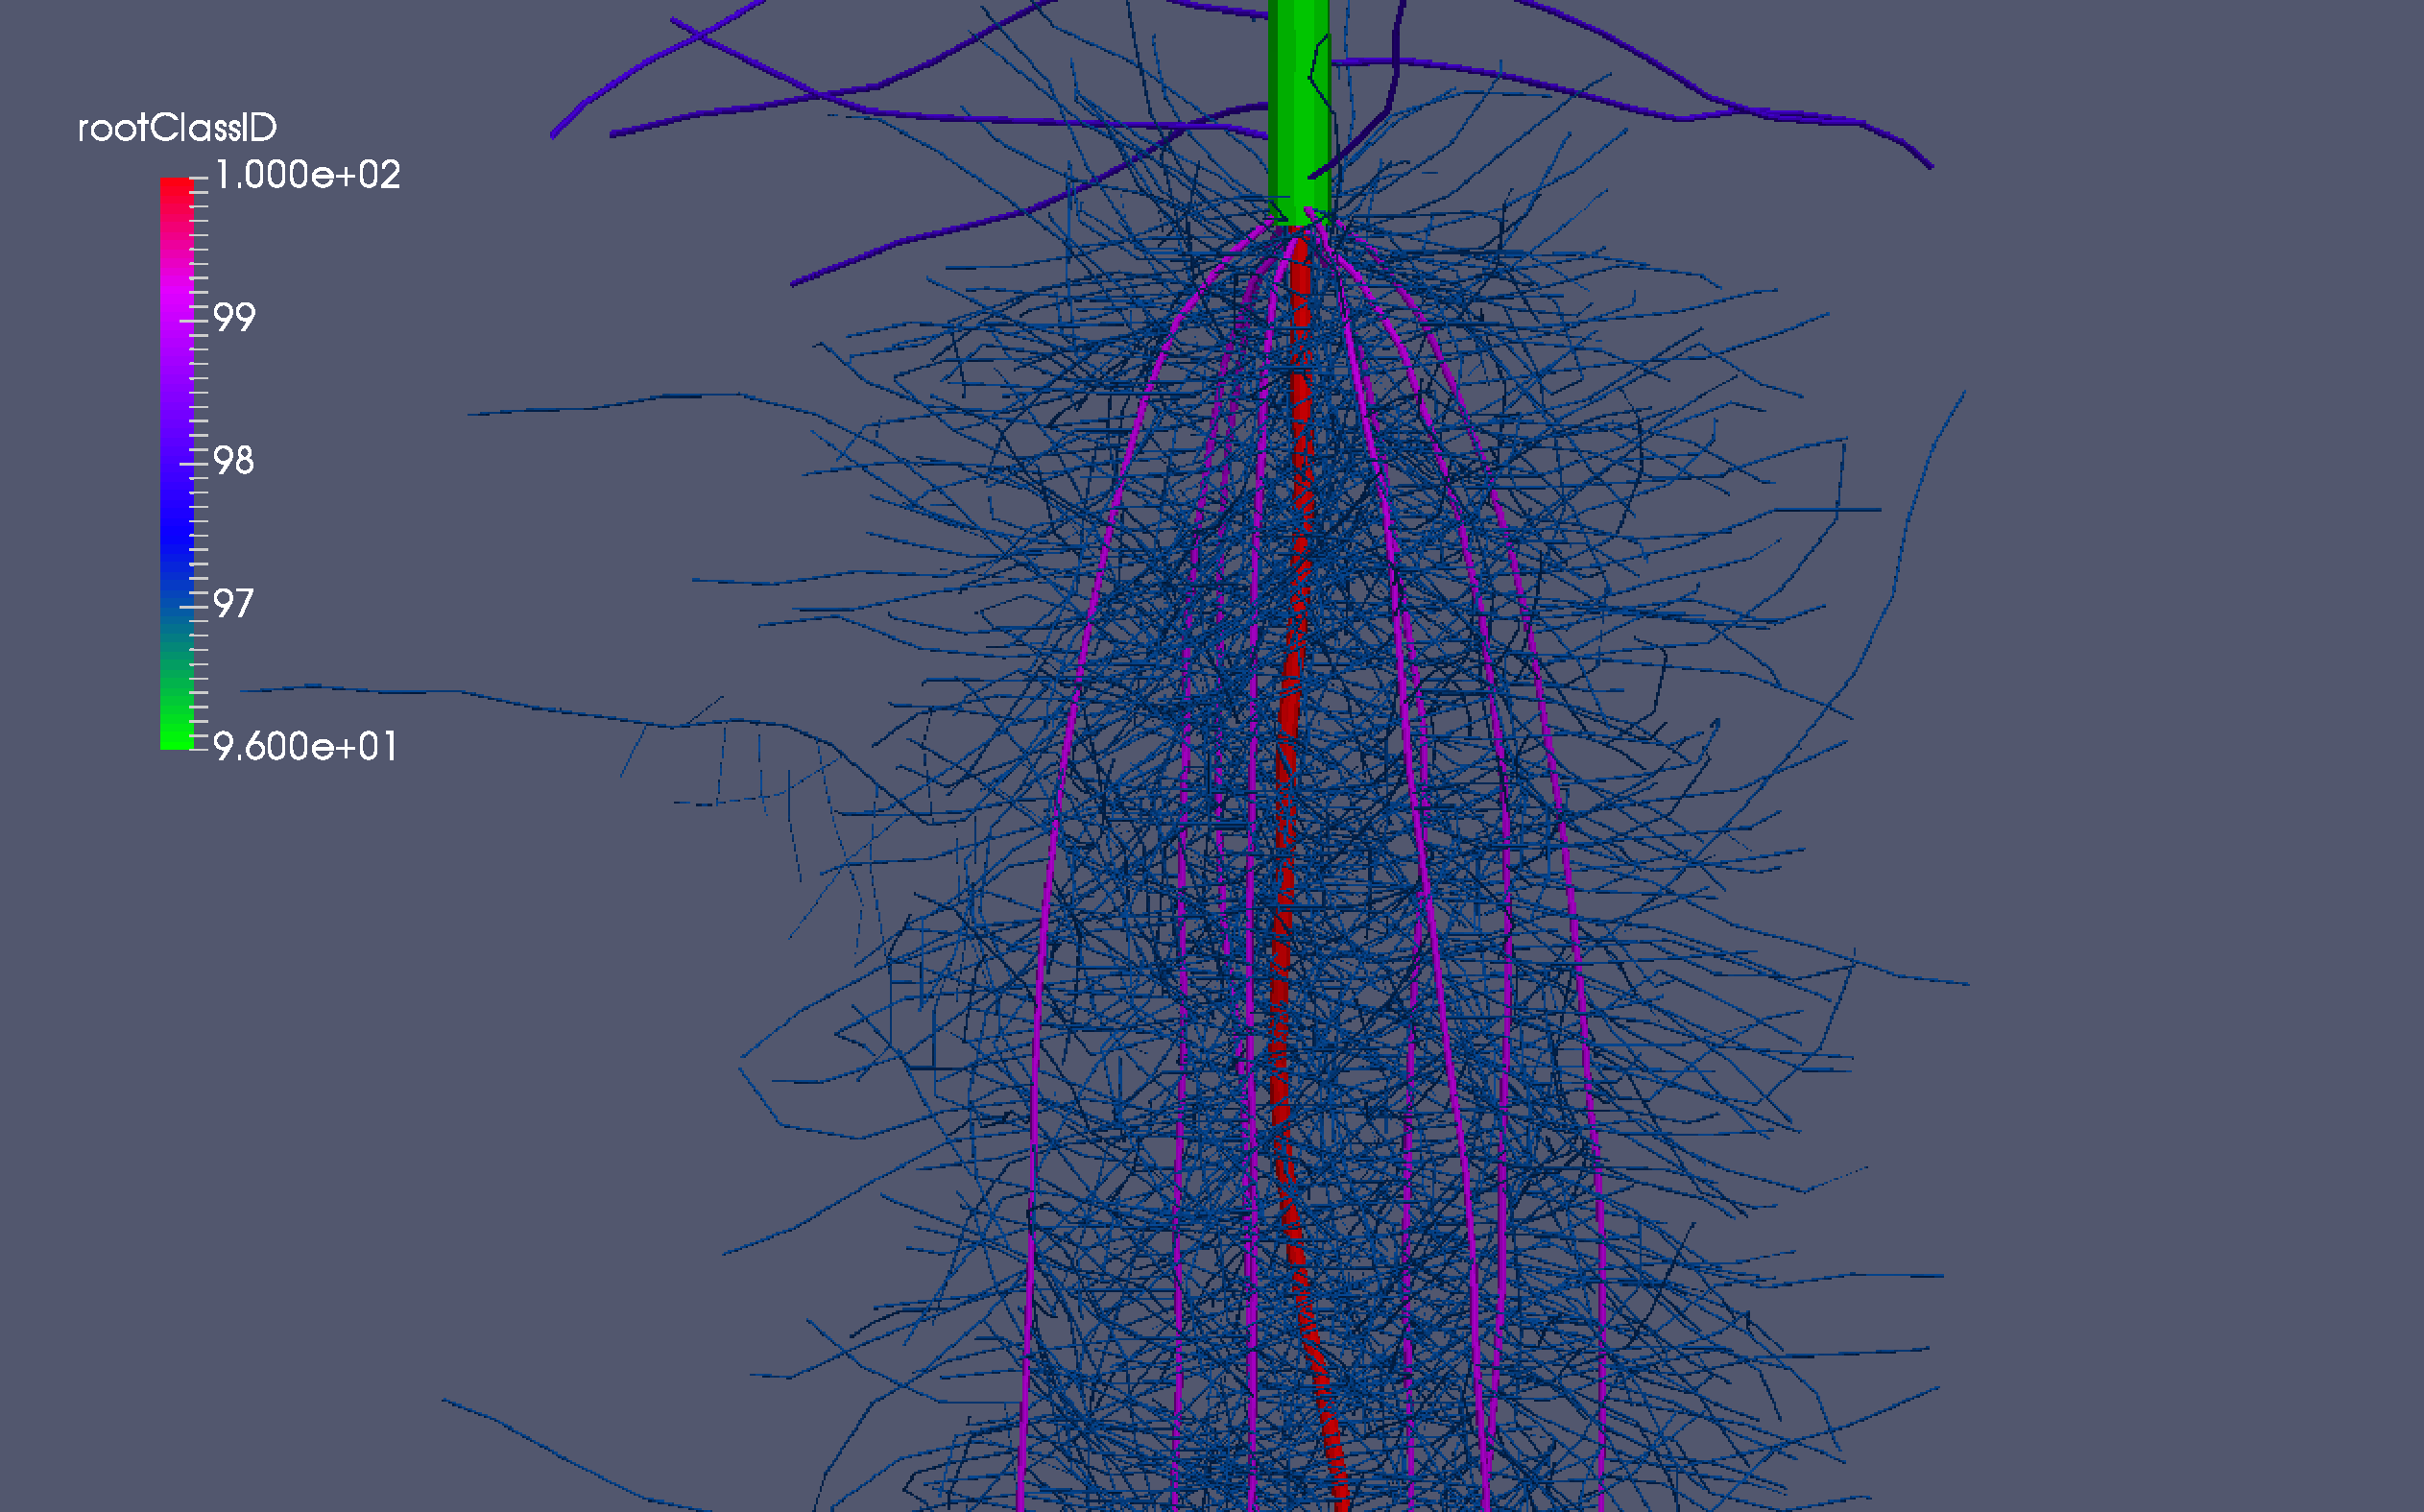
\includegraphics[scale=0.4]{test.pdf}
\caption{A sample root system. The different colours indicate different root classes. The primary root is red, the seminal roots are purple, the hypocotyl is green, the adventitious roots are dark purple and the laterals are blue.}
\end{center}
\end{figure}

%%%%%%%%%%%%%%%%%%%%%%%%%%%%%%%%%%%%%%%
\section{Creating Input Files for OpenSimRoot}\label{Input}

\noindent Since OpenSimRoot aims to simulate many different aspects of root systems, a lot of parameters have to be specified. This means quite extensive input is needed. In this section we will describe the structure of input files and some of the parameters needed to run a simulation. \newline

\noindent As mentioned before, OpenSimRoot does not have a graphical user interface and must be run through the command line (or terminal if you're a linux or mac user). When running OpenSimRoot an xml file with all the input parameters must be specified. For those unfamiliar with xml, it is a markup language similar to HTML. It can be used to store and describe data. In an xml file, information is organized in nested tags, think of them as containers that can store data or other tags. This leads to a hierarchy of tags and data which puts all minimodels in context. For example, each root class will have a tag with subtags containing the different properties of each root class. \newline

\noindent Metadata can also be associated to each tag. In OpenSimRoot, the metadata should always at least include the name. Tags are contained in brackets: \verb| <exampleTag>|. They are closed by either adding a \verb|/| in front of the closing bracket or by repeating the tag with a \verb|/| after the opening bracket. Like this:
\begin{itemize}
\item \verb|<exampleTag/>| 
\item \verb|<exampleTag> nested data </exampleTag>|
\end{itemize} 

\noindent The outermost tag should be \textit{SimulationModel}. The tags in the XML can be of the following types:

\begin{itemize}
\item \textbf{SimulaIncludeFile.} Use this tag to include another XML file. This is useful for keeping your input files (relatively) short and readable. The included file should have \verb|<SimulationModelIncludeFile>| as outer tag.
\item \textbf{SimulaDirective.} Use this to add subtags to an already existing tag. If, for example, one wants to add a property to the primary root in a file different from the one that the primary root is defined in, one would use the tag: 
\begin{verbatim}
<SimulaDirective path="rootTypeParameters/min/primaryRoot">
     <SimulaBase name = "newProperty"\>
<\SimulaDirective>
\end{verbatim}
Here \textit{min} is the plant type.
\item \textbf{SimulaBase.} These are tags that contain other tags, such as \textit{primaryRoot}, \textit{branchList} or \textit{simulationControls}.
\item \textbf{SimulaConstant.} This is used for any kind of fixed parameter in the simulation. Examples are: The total time the simulation should run, the density of roots or the optimal nutrient content of the roots.
\item \textbf{SimulaStochastic.} This is used for any stochastic parameter. In the current version, one can choose from the following distributions: Uniform (both integers and real numbers), normal, lognormal and Weibull.
\item \textbf{SimulaTable.} This tag is used for parameters that change over time, such as the growth rate of the roots or the precipitation.
\item \textbf{SimulaVariable.} Used for variables changing over time calculated using numerical integration. Examples are the actual growth rate of the roots or the water uptake rate. A plugin and an integration function need to be specified.
\item \textbf{SimulaDerivative.} This tag is used for a minimodel coupled to a plugin, which needs to be specified.
\item \textbf{SimulaExternal.} This tag is used for minimodels that are determined by external models, such as the water model. This external model needs to be specified.
\item \textbf{SimulaLink.} This tag is used to link to other minimodels.
\item \textbf{SimulaPoint.} This tag is used for points moving through space, i.e. the growthpoints.
\end{itemize}

%\noindent In addition, one can use the classes described in section \ref{Engine} as XML tags, with the exception of \textbf{SimulaDynamic}, \textbf{SimulaDerivative}, \textbf{SimulaTimeDriven} and \textbf{Database}. 

\noindent To give a feeling for the structure of an xml input file, here is a minimal example xml file

\lstset{language=xml}
\begin{lstlisting}
<?xml version="1.0" encoding="UTF-8" standalone="no"?>
<?xml-stylesheet type="text/xsl" href="xml/treeview.xsl"?>
<SimulationModel name="minTestModel" date="xxx" >
    <SimulaIncludeFile fileName="minTestPlant.xml"/>	
    <SimulaIncludeFile fileName="simulationControlParameters.xml"/>
    <SimulaIncludeFile fileName="templates/plantTemplateMinModel.xml"/>
    <SimulaIncludeFile fileName="plantParameters/min.xml"/>
</SimulationModel>
\end{lstlisting}

\noindent As you can see, other files are referenced here so that it is easy to enable or disable modules. The \textit{minTestPlant.xml} file looks like:

\begin{lstlisting}
<?xml version="1.0" encoding="UTF-8" standalone="no"?>
<SimulationModelIncludeFile>
    <SimulaBase name="minTestPlant" objectGenerator="seedling">
        <SimulaConstant name="plantType" type="string"> 
            min
        </SimulaConstant>	
        <SimulaConstant name="plantingTime"  unit="day" type="Time">
            0
        </SimulaConstant>	
        <SimulaConstant name="plantPosition" type="Coordinate">
            0 -2 0
        </SimulaConstant>
    </SimulaBase>
</SimulationModelIncludeFile>
\end{lstlisting}

\noindent The other files referenced have similar structure. Note that this example is the absolute minimum that OpenSimRoot needs to run. If one wants to simulate geometrical aspects of the roots, the dry weight, water, nutrients or respiration one would need to add several XML files for each of these. To make OpenSimRoot more accessible for new users, sample XML files have been created. These contain the minimum number of parameters and tags needed to run certain modules. This has been done for the geometry, dry weight, water, nitrate, phosphorus and carbon modules. See the directory \verb|OpenSimRoot/OpenSimRoot/Inputfiles|. \newline %add a hyperlink here!

%%\begin{itemize}
%%\item exampleplant
%%\begin{itemize}
%%\item plantType
%%\item plantingTime
%%\item plantPosition
%%\end{itemize}
%%\item simulationControls
%%\begin{itemize}
%%\item integrationParameters
%%\item outputParameters
%%\end{itemize}
%%\item plantTemplate
%%\begin{itemize}
%%\item rootLength
%%\item rootVolume
%%\item rootSurfaceArea
%%\end{itemize}
%%\item shootTemplate
%%\item siblingRootTemplate
%%\begin{itemize}
%%\item dataPoints
%%\item growthpoint
%%\end{itemize}
%%\item hypocotylTemplate
%%\begin{itemize}
%%\item dataPoints
%%\item growthpoint
%%\end{itemize}
%%\item dataPointTemplate
%%\begin{itemize}
%%\item rootDiameter
%%\item rootClassID
%%\end{itemize}
%%\item rootTypeParameters
%%\begin{itemize}
%%\item resources
%%\item shoot
%%\item hypocotyl
%%\begin{itemize}
%%\item rootClassID
%%\end{itemize}
%%\item primaryRoot
%%\begin{itemize}
%%\item rootClassID
%%\item branchlist
%%\item growthRate
%%\end{itemize}
%%\end{itemize}
%%\end{itemize}

\noindent Understanding the structure of these XML files is vital to undestanding the inner workings of OpenSimRoot and required knowledge for anyone who wishes to add new functionality. As seen, the outermost tag is \textit{SimulationModel}. Within these we have \textbf{SimulaBase} tags such as \textit{minTestPlant}, \textit{plantTemplate}, \textit{shootTemplate}, \textit{dataPointTemplate} and \textit{rootTypeParameters}. The \textit{minTestPlant} \textbf{SimulaBase} tells OpenSimRoot to construct a seedling of type \textit{min} at time 0 and position (0,-2,0). If more plants have to be simulated, one would add other \textbf{SimulaBase} tags with as \textbf{objectGenerator} \textit{seedling} and specify the type, planting time and planting position of these other plants. \newline

\noindent The ``simulationControlParameters.xml" file contains the overall settings of the simulation. Examples of these are the total number of days that have to be simulated, or the values that OpenSimRoot should provide as output. \newline

\noindent The \textit{plantTemplateMinModel.xml} file contains the containers that OpenSimRoot will use. An example of this is the \textbf{SimulaBase} \textit{dataPoints} where simroot will store the location of the root segments. Many of these tags are empty to start with, OpenSimRoot only requires them to exist so it can construct the object tree. Another illustration of this is the \textbf{SimulaBase} \textit{branches} where OpenSimRoot will insert new lateral roots. \newline

\noindent Finally, the \textit{plantParameters/min.xml} file contains the numerical values of the parameters OpenSimRoot needs to run. In this minimal example, some of these parameters are the growth rates of the primary root and hypocotyl at different times and the gravitropism of the primary root. Naturally, when more aspects are simulated, more parameters are needed such as the distribution of nutrients in the soil, the precipitation, the transpiration rates of the plant, the leaf area etc. \newline

\noindent It is important to mention here that generally, there is some stochasticity in certain aspects of the simulation like the branching and the growth direction of the roots. If one wants to make simulations reproducible or see the effect of a small change in the code, one has to define a random seed. This can be done using the tag

\begin{verbatim}
<SimulaConstant name="randomNumberGeneratorSeed" type="int"> 1234	</SimulaConstant>
\end{verbatim}

\noindent which should be under the \textbf{SimulaBase} tag \textit{SimulationControls}.
%%%%%%%%%%%%%%%%%%%%%%%%%%%%%%%%%%%%%%%
\section{Writing new modules for OpenSimRoot}\label{Writing}

\noindent Writing a new module for OpenSimRoot is relatively easy, as in principle no other modules need to be changed, provided one knows C++. Being comfortable with using pointers is especially important. Each module consists of one or more minimodels and associated plugins, each of which has to have certain methods and needs to be registered into the database in a specific way. The minimal template for a new plugin is as follows:

\lstset{language=c++}
\begin{lstlisting}
#include "NewPlugin.hpp"
std::string NewPlugin::getName() const{
	return "NewPlugin";
}
NewPlugin::NewPlugin(SimulaDynamic* pSD) :
DerivativeBase(pSD){
}
void NewPlugin::calculate(const Time &t, double &d){
}
DerivativeBase * newInstantiationNewPlugin(SimulaDynamic* const pSD){
	return new NewPlugin(pSD);
}
class AutoRegisterRootLossInstantiationFunctions {
public:
	AutoRegisterRootLossInstantiationFunctions() {
		// register the maker with the factory
		BaseClassesMap::getDerivativeBaseClasses()["newPlugin"] = newInstantiationNewPlugin;
	}
	;
};
static AutoRegisterRootLossInstantiationFunctions p5236245;
\end{lstlisting}

\noindent The header corresponding to this should look like:

\begin{lstlisting}
#ifndef NEWPLUGIN_HPP_
#define NEWPLUGIN_HPP_
#include "../../engine/BaseClasses.hpp"

class NewPlugin: public DerivativeBase{
public:
	NewPlugin(SimulaDynamic* pSD);
	std::string getName() const;
protected:
	void calculate(const Time &t, double &var);
};
#endif
\end{lstlisting}

\noindent Each plugin should have a constructor with as argument a pointer to a \textbf{SimulaDynamic}, \textit{pSD}. This is used as a starting point for navigating around the extensible tree structure. It should also have the methods \textbf{getName} and \textbf{calculate}. The \textbf{getName} method simply returns the name of the plugin. This is used to identify the right classes and to navigate the extensible tree structure. The \textbf{calculate} method will calculate and return the value of the associated minimodel. In the \textit{simulationControlParameters.xml} file (or any other file that contains the relevant parameters) one can specify how often values are written to the output. The minimodels that record global variables will write these to the \textit{tabled\_output.dat} file as specified. \newline

\subsection{The API}\label{API}

\noindent \textbf{Note:} When writing a module, one invariably needs to obtain values from other modules and thus knowing how to navigate the extensible tree structure is essential. We will now explain the most common methods used. Assume that all these methods are called from a \textbf{SimulaBase}-object called \textit{current}.

\begin{itemize}
\item \begin{verbatim} SimulaBase* getParent() \end{verbatim}
This method returns a \textbf{SimulaBase*}, a pointer to the \textbf{SimulaBase} that is the parent of ``current". The method is overloaded and can take a positive integer as input. This will prompt the method to go up this number of steps, so choosing \textbf{2} as input will prompt it to return the `grandparent' instead of the parent, etc.
\item \begin{verbatim} SimulaBase* getChild(const std::string& childName) \end{verbatim}
This method returns a \textbf{SimulaBase*} pointing to the child of ``current'' which is called ``childName". Of course, if ``current" does not have a child with that name, it will lead to an error message. This is why the following method exists.
\item \begin{verbatim} SimulaBase* existingChild(const std::string& childName) \end{verbatim}
This method works similarly to the above one, except that if no child with the given name exists, it returns a null pointer. If one wants to get a value from an optional module, on the condition that it is being used, this method is used instead of the previous one.
\item \begin{verbatim} SimulaBase* getSibling(const std::string& siblingName) \end{verbatim}
This method is equivalent to 
\begin{verbatim} getParent()->getChild(const std::string& siblingName) \end{verbatim}
but obviously preferable. The method
\begin{verbatim} SimulaBase* existingSibling(const std::string& siblingName) \end{verbatim}
works just like one expects.
\item \begin{verbatim} SimulaBase* getNextSibling() \end{verbatim}
This method returns a pointer to the next sibling in the lexicographical ordering. This is useful for iterating over all the datapoints of a root in order, as they are created in lexicographical order.
\item \begin{verbatim} SimulaBase* getPreviousSibling() \end{verbatim}
This method returns a pointer to the previous sibling in the alphabetical ordering.
\item \begin{verbatim} SimulaBase* getFirstChild() \end{verbatim}
This method returns a pointer to the first child of ``current" in the alphabetical ordering. Useful for the start of an iteration over all children.
\item \begin{verbatim} SimulaBase* getLastChild() \end{verbatim}
This method returns the last child in the alphabetical ordering.
\item \begin{verbatim} void getAllChildren(SimulaBase::List& childrenList) \end{verbatim}
A \textbf{SimulaBase::List} object is a vector of \textbf{SimulaBase*} objects, so a vector of pointers. This method copies the list of all children of ``current" to childrenList. This is useful when iteration over elements is needed.
\item \begin{verbatim} std::string getName() \end{verbatim}
This method returns the name of the SimulaBase object from which it's called, in this case that would be ``current".
\item \begin{verbatim} std::string getPath() \end{verbatim}
This method returns a string that describes the path from the origin to ``current". Can greatly improve the usefulness of error messages. For example, the path to the first datapoint of the primary root could be: \verb| origin/examplePlant/plantPosition/primaryRoot/dataPoints/dataPoint00000 |
\item \begin{verbatim} SimulaBase* getPath(const std::string& path) \end{verbatim}
This method returns a pointer to the SimulaBase object specified by ``path". If unsure if this object exists, one can use
\begin{verbatim} SimulaBase* existingPath(const std::string& path) \end{verbatim}
\end{itemize}

\noindent To navigate the extensible tree structure (ETS), one obviously has to know its topology. To get an overview of the structure of the ETS, turn on the \textit{modelDump}-option. This will write the ETS at the specified times to an XML file. It can be viewed in any internet browser. One might have to delete the second line, which is shown below, on some systems.

\begin{verbatim}
<?xml-stylesheet type="text/xsl" href="XML/outlineview.xsl" ?>
\end{verbatim}

\noindent It is advisable to not do a model dump for simulations that have run for more than a couple of days, the output file might turn out to be several hundreds of MB in size.

%\noindent As an example, consider a module that calculates the volume of a root segment. It will instantiate an object attached to each datapoint and the calculate method will return the root volume when called. It calculates this from the length and diameter of the root segment. This code could, as an example, look like this:
%
%\begin{verbatim}
%void calculate(const Time &t, double &segmentVolume){
%     double segmentLength, segmentDiameter;
%     pSD->getParent()->getChild("rootSegmentLength")->get(t,segmentLength);
%     pSD->getSibling("rootSegmentDiameter")->get(t,segmentDiameter);
%     segmentVolume = segmentLength*segmentDiameter*segmentDiameter/4*M_PI;
%}
%\end{verbatim}
%
%\noindent Of course most modules use parameters that are read in from the input files, check if certain conditions, such as other object existing, are true and do more complicated computations, but this basic example should showcase enough of the structure to allow you to begin writing your own module. It should also be noted that the root segments are actually conical frustrums, not cyllinders so this formula does not calculate the segment volume!


%\section{Module Guide}
%
%\noindent In this section we will describe the core modules, which have associated templates. For each module we will briefly describe what it does, what dependencies it has, if any, the input parameters needed to run it and any optional features. Using these descriptions and the templates found in the \href{https://gitlab.com/rootmodels/OpenSimRoot}{OSR online repository} users should be able to create input files from scratch, provided they have the necessary input parameters. This section is a work in progress.

\section{Acknowledgements}

We would like to acknowledge the developer of OpenSimRoot, Dr. Johannes Postma, whose comments and corrections were essential for this manual. We would also like to acknowledge Dr. Nathan Mellor, discussions with whom helped clarify many of the aspects of OpenSimRoot we discussed. Finally we would like to thank Prof. Markus Owen for his extensive feedback.

\bibliographystyle{plain}
\bibliography{Database}

\end{document}